\documentclass[../lecture4-functions.tex]{subfiles}

\begin{document}

\section{Function Call and Execution}

% -------------------------------------------------------------------

\begin{frame}[fragile]{Function Call and Execution}
    The function definition is entirely passive. By itself it does nothing unless instructed to execute. This is done by a statement in the main program called the \textbf{function call}. \newline

    For example the statement:
    \begin{cppcode}[lastline = 1, fontsize=\footnotesize]
result = factorial(number);
    \end{cppcode}

    calls the function \mintinline{cpp}{factorial()} and passes a copy of the value stored in the variable, number. When the function is called, computer memory is allocated for the parameter, \verb|number| and the value passed is copied to this memory location. Memory is also allocated to the (local) variables \verb|factorial| and \verb|ii|. The statements of the function are then executed and assign a value to the variable \verb|factorial|. The return statement passes this value back to the calling function. The memory allocated to the parameters and local variables is then destroyed. The value returned is assigned to the variable on the left-hand side, result, in the expression used to call the function. The net effect of executing the function in our example is that the variable \verb|result| has been assigned the value of the factorial of number.
\end{frame}

% -------------------------------------------------------------------

\begin{frame}[fragile]{Example Execution}
    A function can be called any number of times from the same or different parts of the program. It can be called with different parameter values (though they must be of the correct type). \newline

    For example the following fragment of code can be used to print out the factorials of the first 10 integers: \newline

    \begin{cppcode}[lastline = 5]
for(ii = 1; ii <= 10; ii++)
{
    result = factorial(ii);
    cout << ii << "! = " << result << endl;
}
    \end{cppcode}
    and
    \begin{cppcode}[lastline = 1]
binomialCoefficient = factorial(n) / (factorial(k) * factorial(n - k));
    \end{cppcode}

    can be used to compute the binomial coefficient \( \frac{n!}{k!(n - k)!} \)
\end{frame}

% -------------------------------------------------------------------

\begin{frame}[fragile]{Programming memes for those who don't know what a binomial coefficient is - all good I forgot aswell}
    \begin{center}
        \makebox[\textwidth]{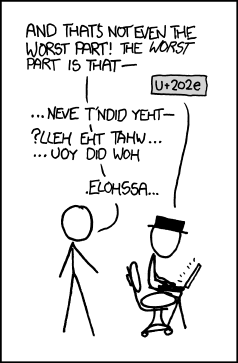
\includegraphics[width=0.80\paperwidth,height=0.80\textheight]{graphics/xkcd-rtl.png}}
    \end{center}
\end{frame}

% -------------------------------------------------------------------

\end{document}
